\section{Externe Schnittstelle}
\label{sec:implementation:externalApi}
Neben der Interaktion mit Benutzern der \textit{TyrolSky}-Anwendung über die \textit{API}-Komponente, wird auch eine Kommunikation mit einem Fremdsystem benötigt. Um Abbuchungen an einem Konto vorzunehmen, wird, wie im Anforderungskatalog unter Abschnitt \ref{sec:Eruierung:technicalRequierements} gefordert, eine externe Anwendung angebunden. Diese Bankenanwendung operiert als eigenständige Anwendung und simuliert eine Bankenschnittstelle um Kontoabbuchungen von Kunden vorzunehmen. Die Simulationsanwendung selbst ist im nachfolgenden Kapitel \ref{subsec:implementation:bankApi} genauer beschrieben. \\
Der bereits in Abschnitt \ref{subsub:implementation:ChargingCoordinator} beschriebene Buchungskoordinator verteilt Abbuchungstransaktionen, mithilfe von \textit{Sharding}, innerhalb des Clusters auf verschiedene Nodes. Jede Transaktion benötigt jedoch eine Kommunikation mit der Bankenschnittstelle, um die Transaktion durchzuführen und sie mit dem Bankensystem abzugleichen. \\
Dazu wird auf jedem Node der Buchungen durchführen kann, das sind alle Nodes mit der Rolle \textit{Domain-Service}, ein \textit{Banking-Actors} gestartet. Dieser ist anschließend für die Kommunikation mit der Bankenanwendung zuständig. \\
Möchte nun eine Transaktion eine Kommunikation mit der Bankenanwendung starten, sendet diese einen Befehl in Form einer Nachricht an den \textit{Banking-Actor}. Der \textit{Banking-Actor} befindet sich auf dem gleichen Host wie der Transaktions-Actor. Der Befehl an den \textit{Banking-Actor} enthält Informationen über die gewünschte Kommunikation mit der Bankenschnittstelle. Wird während der Kommunikation zur Bank der betroffene Transaktions-Actor durch \textit{Sharding} verschoben, betrifft dies nicht den Banking-Actor selbst, da dieser fix auf jedem Host als eigene Actor-Instanz vorhanden ist. 
\subsection{Banken-API}
\label{subsec:implementation:bankApi}
Für die Anbindung einer externen Bank wurde eine eigene Software geschrieben, die eine simulierte und einfach gehaltene Bankenschnittstelle zur Verfügung stellt. Die \textit{BankChargingAPI} ist komplett getrennt von der restlichen Implementierung der \textit{TyrolSky}-Anwendung und kann über eine eigene \textit{REST}-Schnittstelle angesprochen werden. \\
Die Kernaufgabe dieser Bankensimulation ist es, Bankkonten zu verwalten. Dazu werden in einer relationalen Datenbank Kontoinformationen abgebildet. Dabei hat jedes Konto einen Namen sowie einen aktuellen Guthabenstatus. Für die Bankentransaktionen, nicht zu verwechseln mit den Transaktion innerhalb der \textit{TyrolSky}-Anwendung, wird eine eigene Tabelle geführt, welche Informationen über jede bearbeitete Transaktion enthält. Die Transaktion enthält Informationen über den eigenen Status sowie den Transaktionsbetrag. Über die Schnittstelle kann auch der Status einer Transaktion abgefragt werden. Diese Transaktionsstatus-Abfrage wird auch von der \textit{TyrolSky}-Anwendung verwendet um die eigene Flugbuchung zu kontrollieren, beschrieben unter Abschnitt \ref{subsub:implementation:ChargingCoordinator}. \\
Für die Implementierung der Simulationsanwendung wurde auf eine \textit{SQL-Datenbank} zurückgegriffen. Jeder Zugriff auf die Datenbank erfolgt in einer Transaktion mit dem strengen Transaktionslevel \textit{Serializable}, wodurch keine Inkonsistenzen der Kontoinformationen entstehen können \citep{adya2000generalized}. Durch die Transaktionstabelle ist eine Nachvollziehbarkeit der getätigten Transaktionen möglich. \\
Die Simulationsanwendung \textit{BankChargingAPI} bietet folgende Schnittstellen für die \textit{TyrolSky}-Anwendung an:
\begin{itemize}
  \litem{ChargeAccount}
    Mit Angabe des gewünschten Kontos sowie dem abzubuchenden Betrages wird eine Transaktion gestartet. Für den Aufruf wird eine Transaktionsnummer angegeben, mit der später der Status der Transaktion abgefragt werden kann.
  \litem{GetTransactionStatus}
    Durch Angabe der Transaktionsnummer wird der aktuelle Status der Transaktion zurückgegeben. 
\end{itemize}
Durch die Aufteilung in zwei Methoden ist es möglich im Fehlerfall Transaktionsinformationen nicht zu verlieren. Wird beim Aufruf der \textit{ChargeAccount}-Schnittstelle kein Ergebnis zurückgeliefert, kann der Status über \textit{GetTransactionStatus} zu einem späteren Zeitpunkt abgefragt werden.

\section{Testapplikation}
\label{subsec:implementation:TestApplikation} 
Die \textit{TyrolSky}-Anwendung bietet eine Schnittstelle für Endbenutzer an, mit der die Anwendung bedient werden kann. Um eine größere Menge an Benutzern und somit Anfragen zu simulieren wird eine eigene Testapplikation benötigt. Diese bietet die Möglichkeit eine Vielzahl an Flügen zu reservieren sowie zu buchen. Für jede Anfrage an das \textit{TyrolSky}-System wird die Anfrage protokolliert und der Rückgabewert der Anfrage abgespeichert. Dadurch können nach einem Testdurchlauf die Resultate eingesehen und mit dem Zustand des getesteten Systems verglichen werden. \\
Die Umsetzung der Testapplikation fordert einen hohen Grad an Parallelisierung, da gleichzeitig eine Vielzahl an Anfragen an das System gestellt werden sollen. Aufgrund der Anforderung an eine bestmögliche Parallelisierung wird die Anwendung mit dem Actor-Model, das für parallelisierte Anwendungen konzipiert wurde, siehe dazu \ref{actor:parallelism}, realisiert. Wie die Implementierung der externen Bankenanwendung ist auch die Testapplikation eine vollständig eigenständige Anwendung, welche keinen Zusammenhang mit der Implementierung der \textit{TyrolSky}-Anwendung besitzt. \\
Jede Anfrage, die zum testenden System durchgeführt wird, ist in einer Datenbanktabelle protokolliert. Dabei werden Informationen zur Anfrage selbst, wie Flugnummer, Flugdatum und Passagierinformation sowie Informationen zur Buchungs selbst abgespeichert. Der genaue Aufbau der Tabelle \textit{StressTest}, welche alle Informationen über eine Anfrage enthält, ist aus Abbildung \ref{fig:implementation:stressTestDbSchema} zu entnehmen.
\begin{figure}
  \centering
  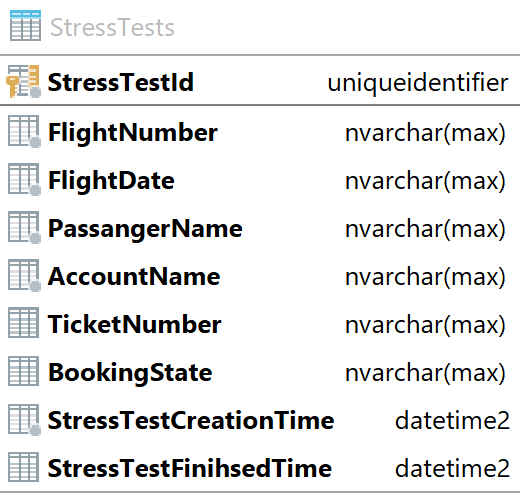
\includegraphics[width=0.4\linewidth]{gfx/implementation/stressTestDbSchema}
  \caption{Datenbankschema für die Testapplikation der \textit{TyrolSky}.}
  \label{fig:implementation:stressTestDbSchema}
\end{figure} 

Die Testanwendung wird in Form einer Konsolenanwendung ausgeführt. Dabei kann beim Start der Anwendung über Parameter angegeben werden, welche Flüge zu welchem Ausmaß gebucht werden sollen. Die Anwendung startet anschließend die entsprechenden Schritte, um Flüge zu buchen. 

\subsection{Ablauf eines Testes}
Nach dem Starten der Konsolenanwendung werden die übergebenen Parameter ausgelesen und das Actor-System für den Testlauf erzeugt. Anschließend wird die vom Tester geforderte Anzahl an Buchungen durchgeführt. Für jede Buchung wird ein eigener Buchungs-Prozess gestartet, welche in der Tabelle \textit{StressTest} abgebildet sind. Dabei wird zuerst versucht, ein Ticket zu reservieren. Konnte eine Reservierung erfolgreich durchgeführt werden, versucht die Anwendung diese Reservierung abschließend zu buchen.
Die für die Buchung benötigten Kontoinformationen werden ebenfalls in der Tabelle \textit{StressTest} zur aktuell getesteten Buchung abgespeichert. Die Testanwendung fragt nach der Buchungsaufforderung, das zu testenden System nach dem Buchungsresultat, bis dieses einen endgültigen Buchungsstatus zurückliefert. \\
Die einzelnen Buchungsjobs werden dabei nicht alle gleichzeitig gestartet. Alle zwei Sekunden beginnen zehn neue Jobs, diese laufen jedoch parallel bis zur Fertigstellung des Jobs weiter. Die Gesamtanzahl an Jobs wird über die Parameter der Anwendung gesteuert. Ist die Testanwendung beendet, kann das Resultat in der Datenbank abgefragt werden. Weiters können durch die Angabe der Kontoinformationen die Resultate mit der \textit{BankChargingAPI}-Anwendung sowie mit den entsprechenden Passagierlisten der \textit{TyrolSky}-Anwendung verglichen werden.

\subsection{Parameter Beschreibung}
Für die Steuerung und Parametrisierung der \textit{TyrolSky}-Testapplikation können folgende Parameter zum Starten der Konsolenanwendung angewandt werden:

\begin{itemize}
  \litem{NumberOfBookings} Gesamtanzahl der zu buchenden Tickets
  \litem{FlightsToBook} Angabe einer Liste an verschiedenen Flugnummern, die gebucht werden sollen
  \litem{DateRangeStart und DateRangeStop} Start- und Enddatum für den Zeitraum, in der ein Flug stattfinden soll
  \litem{ChargingAccounts} Fiktive Bankkonto-Informationen, mit denen die Flüge bezahlt werden sollen
\end{itemize}
Die Testanwendung versucht anschließend die angegebene Anzahl an Tickets zu reservieren sowie zu buchen. Dabei wird für jedes Ticket zufällig ein Datum sowie eine zufällige Flugnummer ausgewählt. 
